\subsection{Exploratory factor analysis}
\label{sec:analisis-factorial}

Factor analysis complements PCA (\cref{sec:pca}) by separating the variance
shared among variables from the variance specific to each. For each
standardized variable,
\begin{equation}
  z_j=\sum_{k=1}^{3}\lambda_{jk}f_k+\varepsilon_j,
  \qquad h_j^2=\sum_{k=1}^{3}\lambda_{jk}^2.
  \label{eq:af-modelo}
\end{equation}
The $f_k$ are latent factors, and the loadings $\lambda_{jk}$ give the
magnitude and direction of their association with each variable. With
orthogonal factors of unit variance, the communality $h_j^2$ is the
proportion of variance explained; the uniqueness $1-h_j^2$ captures the
specific part and the error.

\paragraph{Adequacy and extraction}
The initial diagnosis uses 15 predictors and 16,028 complete observations
from 2021--2024. Bartlett's test rejects the absence of correlations
($p<0.001$), although temporal and spatial dependence limit this test. The
initial KMO of 0.647 indicates mediocre adequacy. \texttt{NOX\_06\_09} is
removed because of its redundancy with NO and NO2 (VIF of 45.73). On the
remaining 14 variables, Velicer's MAP suggests three factors, versus seven
from parallel analysis; MAP is adopted for parsimony, and the discrepancy is
kept as a limitation.

Iterated principal axis extraction produces an inadmissible communality of
1.093 for \texttt{RH\_min\_diurna}; this variable is removed and mean
humidity is kept. The final block of 13 predictors reaches a KMO of 0.677
and a maximum VIF of 2.54, with no communalities above one. Three factors are
retained and varimax is applied to ease their interpretation through
orthogonal axes (\cref{fig:af-diagrama}).

\begin{figure}[pos=t]
  \centering
  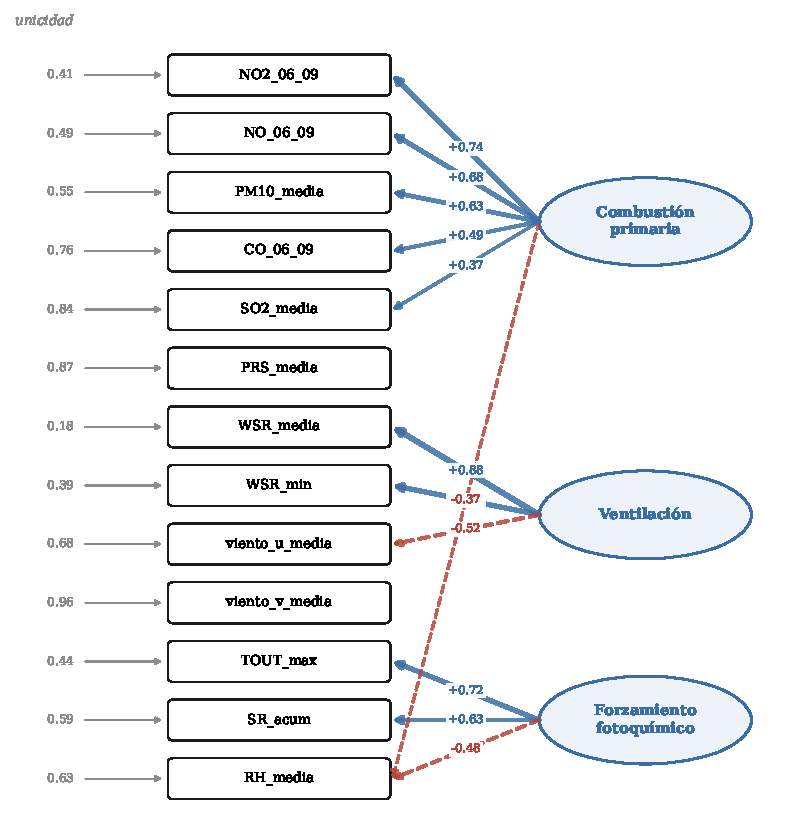
\includegraphics[width=0.92\linewidth]{af_diagrama_cargas.pdf}
  \caption{Varimax loadings with $|\lambda|\geq0.30$. Solid arrows: positive
    associations; dashed: negative. Gray values indicate uniquenesses.}
  \label{fig:af-diagrama}
\end{figure}

\paragraph{Interpretation}
The factors explain 40.3\,\% of the total variance of the 13 predictors.
\emph{Primary combustion} (15.7\,\%) groups NO2 (0.74), NO (0.68), PM10
(0.63), CO (0.49) and SO2. \emph{Ventilation} (14.5\,\%) gathers mean and
minimum wind speed, with loadings of 0.88 and 0.77, and the zonal component
($-0.52$). \emph{Photochemical forcing} (10.1\,\%) combines maximum
temperature (0.72), cumulative radiation (0.63) and mean humidity ($-0.48$):
warm, sunny, dry days. Pressure has a communality of only 0.13, so the name
ventilation is more accurate than attributing an anticyclonic mechanism to
the factor.

Three choices that were tried and discarded along the way ---Horn's parallel
analysis, maximum likelihood extraction and oblique rotation--- are
documented in \cref{sec:tecnicas-descartadas}.

\paragraph{Fit and scope}
The root mean square residual of the reconstructed correlations (RMSR) is
0.0555; 26 of 78 pairs retain absolute residuals greater than 0.05. The fit
is reasonable but partial. Bartlett scores, applied to 2025 with training
weights, have VIFs close to 1.01 and a maximum absolute correlation of 0.097.
That is why they, rather than the PCA scores, are the predictors of the
models of \cref{sec:clasificacion_tecs}, where the comparison is reported.

The three factors reappear in 2025 with Tucker congruence coefficients of
0.973 for combustion, 0.939 for ventilation and 0.924 for photochemistry: the
structure is stable outside the fitting period. The factor score determinacy
(correlation between score and factor) is 0.880, 0.918 and 0.833;
photochemical forcing shares 69\,\% of its variance with the factor it
represents, and the rest is estimation error. The mediocre KMO and the
Box--Cox transformation estimated on the full period remain as caveats. The
factors describe associations; without measurements of volatile organic
compounds they cannot establish ozone formation mechanisms.
